 %%
    \begin{figure}[tbp]
        \centering
        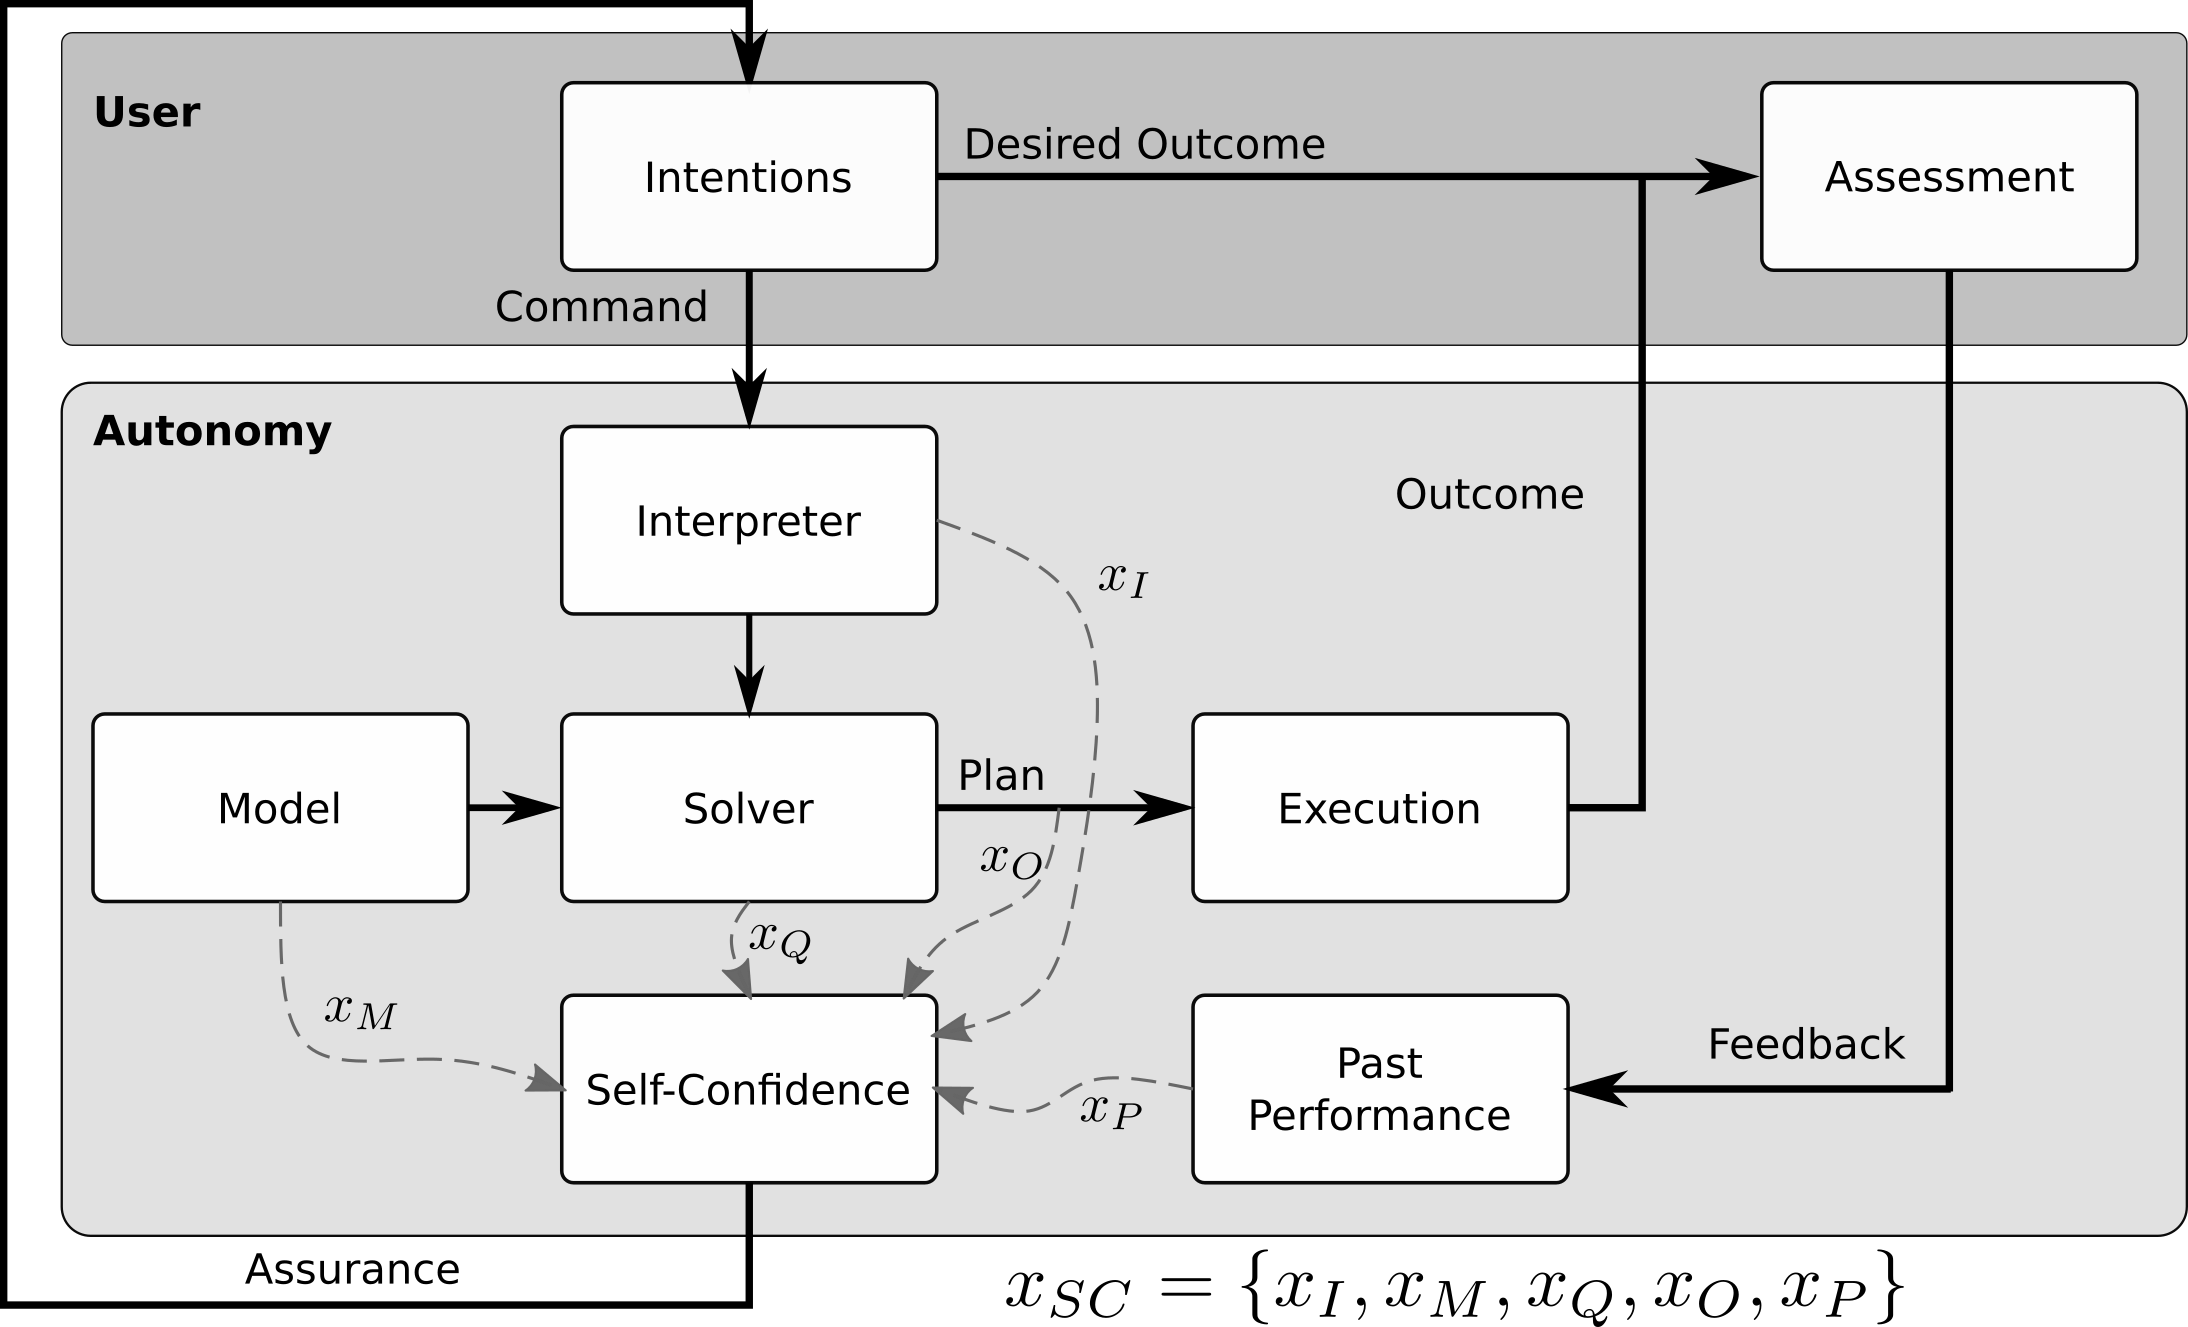
\includegraphics[width=0.7\linewidth]{Figures/FaMSeC.png}
        \caption{Factorized Machine Self-Confidence (\famsec) information flow}
        \label{fig:famsec}
    \end{figure}
    
    %%\nisar{trim/simplify and re-arrange and absorb first part of this section into background section for famsec set up...then need to decide how to split up presentation of two factors...adjust abstract/intro to be consistent...}
\subsubsection{Self-confidence Factorization and Calculation} \label{sec:self-confidence}

    We briefly review and explore an algorithmic approach known as \textit{Factorized Machine Self-confidence (\famsec{})} for assessing and communicating machine self-confidence \cite{Aitken2016-cv, Aitken2016-fb}. 
    %This process-driven approach endows an APS with a mechanism to score how well-suited its decision-making ability is to a task at hand, based on known factors that influence the quality of its reasoning. 
    %%We briefly review the work developed in \cite{Aitken2016-cv, Aitken2016-fb} to highlight: (i) a set of principles, definitions, and relations that govern the  `arithmetic of machine self-confidence' as a function of task, environment, system realization, and context (i.e. independent of algorithmic APS implementation), and (ii) variables, representations and operations for computing concrete quantitative self-confidence assessments for APS implemented with MDPs. 
    %
    %We initially address these issues for APS that are primarily defined by capabilities for dynamic decision-making and planning under uncertainty. This approach provides a pathway to developing firm initial mathematical and computational bases for addressing (i) and (ii) via the rich set of analytical and computational features inherent to the MDP model family. %Insights developed along these lines can provide the basis of future work for formulating self-confidence computation strategies, other important planning model families, and APS capabilities that are formally related to decision making under uncertainty, such as dynamic learning and partially observable planning with sensing and perception. 
    %After reviewing a computational framework for self-confidence assessment that relies on assessing individual factors involved with solving MDP-based planning and decision-making problems, \brett{need to tweak this paragraph a bit to reflect the reduced scope of the paper. }we consider how one of these factors (related to the quality of a given MDP policy solver) can actually be computed, building on insights derived from calculation and analysis of another factor (related to intrinsic task difficulty) examined in other work. 
    %
    %\subsection{The \famsec{} Framework }
    %The approach presented here adopts and builds on the \emph{Factorized Machine Self-Confidence (\famsec)} framework developed in ref. \brett{FAT* paper \cite{Israelsen2018-qz}} and \cite{Aitken2016-cv,Aitken2016-fb}. 
    The key idea behind \famsec{} is to represent and compute self-confidence as a traceable multi-factor function, which combines shorthand assessments of where and when operations and approximations inherent to model-based autonomous decision-making are expected to break down. As with the self-confidence reporting strategy developed in \cite{Hutchins2015-if}, this captures metrics than an expert designer would use to assess the correctness and quality of an autonomous decision-making system, accounting for variations in task, environment, system implementation, and context. However, unlike \cite{Hutchins2015-if}, \famsec{} allows an APS to automatically generate its own holistic assessments of self-confidence, i.e. without the need for a human designer/expert to specify a priori how self-confident a system ought to be given such variations. %%(which can be cumbersome, if not impossible, to fully account for in practical applications). 
    
    Figure \ref{fig:famsec} illustrates \famsec's notional overall self-confidence scoring mechanism. This uses a set of \emph{self-confidence factors} (dashed lines) that are derived from core algorithmic decision-making components (white boxes in the `Autonomy' block). The total self-confidence score can be mapped onto an arbitrary scale, e.g. -1 to +1 for the sake of discussion, where -1 gives a shorthand indication of `complete lack of confidence' (i.e. some aspect of task, environment, or context falls completely outside the system's competency boundaries), and +1 indicates `complete confidence' (i.e. all aspects of task, environment, and mission context are well within system's competency boundaries). As will be shown later, the scales for each factor need not all be the same and can carry slightly different qualitative interpretations, as long as a clear sense of `confidence direction' (i.e. degree of self-trust) can be established for each.
    
    Ref. \cite{Aitken2016-cv} considers five general factors that contribute to a `total self-confidence score', which notionally maps the combined set of factors into an overall confidence report:
    1) \xI---\textit{\textbf{interpretation of user intent and task}}: to what extent were the user's intentions properly understood and translated by the autonomous system into context-appropriate mission specifications and tasks?; 
    2) \xM---\textit{\textbf{model and data validity}}: are the agent's learned and/or assumed models, and associated training data used for decision-making `good enough' proxies for the real world?; 
    3) \xQ---\textit{\textbf{solver quality}}: are the approximations and learning-based adaptations used by the system for solving decision-making problems appropriate for the given mission and model?; 
    4) \xO---\textit{\textbf{expected outcome assessment}}: do the sets of possible events, rewards, costs, utilities, etc. for a particular decision lead to a desirable landscape of possible outcomes?; and 
    5) \xP---\textit{\textbf{past history and experiences}}: what can be gleaned from the system's own experience and other available information for past problem instances? %%\brett{refer to \cite{Israelsen2018-qz} for more detail if we feel we need it}

    Since the overall self-confidence mapping is heavily dependent on application, context, and desired levels/types of user-autonomy interaction, this work assumes for simplicity that the overall mapping consists of a direct report of all or some fixed subset of the component factors, e.g. \xSC. 
    Furthermore, the five factors considered here are neither exclusive nor exhaustive. For example, the factors developed by \cite{Aitken2016-cv,Aitken2016-fb} are primarily aimed at self-assessment \emph{prior} to the execution of a particular task, whereas it is conceivable that other self-confidence factors could be included to account for in situ and post hoc self-assessments. For simplicity, attention is restricted to the a priori task self-assessment case. 

\subsubsection{Revisiting Donut Delivery}
We will use the Donut Delivery problem to examine two core questions: (i) how should the factors be expected to behave under different conditions (independently of how they are actually calculated)?, and (ii) how should any one these factors actually be calculated?

For (i), we can first consider what kinds of trends, `boundary conditions', and which interactions are expected for the various factors if we are given some class of solver for the underlying ADT motion planning problem. For instance, if the problem were modeled and encoded as a discrete-time/discrete-space MDP, then sampling-based Monte Carlo solvers could be used to find an approximately optimal policy $\pi$ \cite{Browne2012-lj}, which would map joint ADT-MG state information onto specific actions to maximize the ADT's expected cumulative reward. Figure \ref{fig:trendsBCs} shows some expected behaviors for the \famsec{} factors for such a solver, as a function of task, environment, system, and context, assuming again an arbitrary finite range of -1 (total lack of confidence) to +1 (complete confidence). For instance, \xQ{} would be expected to increase/decrease as the number of samples used by the Monte Carlo solver to approximate $\pi$ increased/decreased. Similar trends can also be derived for other solver types.  %\nisar{mention about traceability/drill down basis here?}
\begin{figure}[tbp]
    \centering
    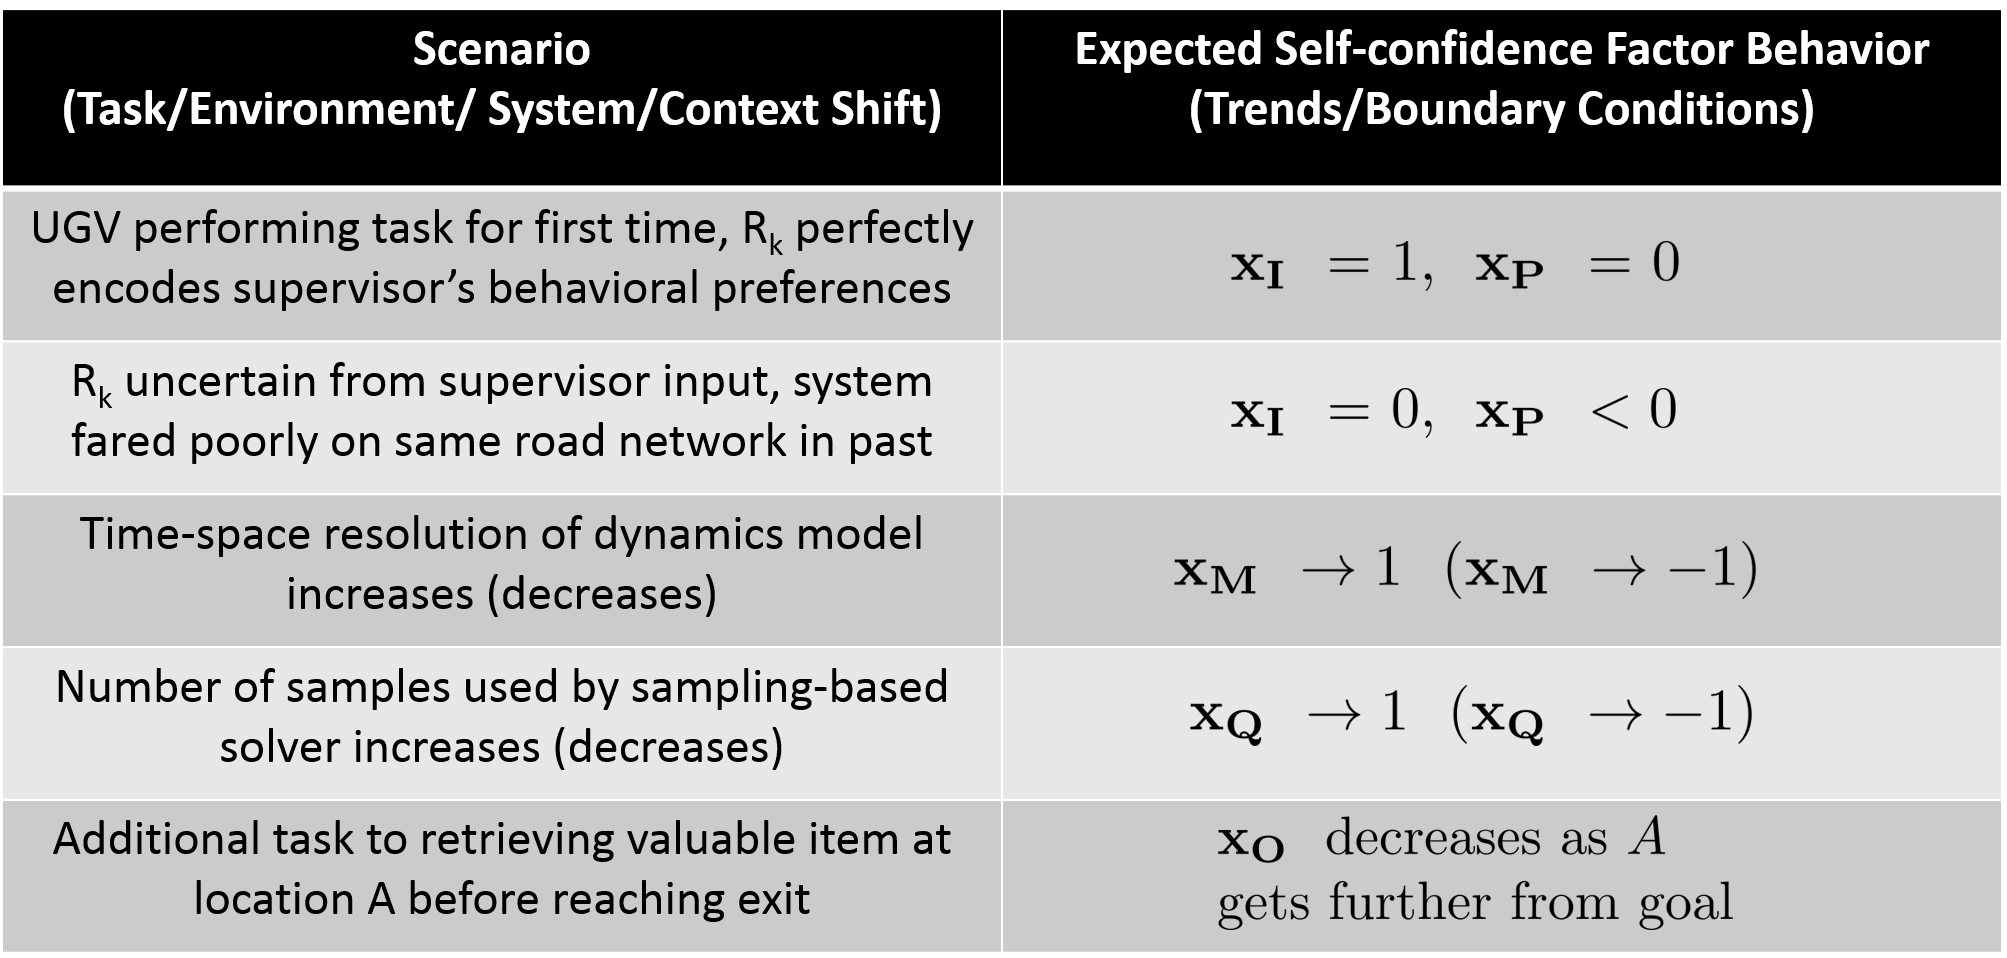
\includegraphics[width=0.65\linewidth]{Figures/scTrendsBoundaryExample_2generic.png}
    \caption{Notional \famsec{} behaviors for Donut Delivery problem.}
    \label{fig:trendsBCs}
\end{figure}

With this in mind, an important issue to consider for addressing (ii) is that the factors can depend on each other in complex ways. A logical simplifying assumption for initial algorithm development is to consider cases where we can ignore the interactions between factors. This is equivalent to examining each factor along `boundary conditions' where other factors do not change and thus have little/no contribution to the overall self-confidence score. 
For example, ref. \cite{Aitken2016-cv} developed an approach to compute \xO{} for infinite horizon MDP planning, assuming the boundary conditions \xM$=+1$ (perfectly known problem/task model), \xI $= +1$ (perfectly interpreted user task command and reward function $R_k$), \xQ$=+1$ (optimal policy $\pi$ known and available), and \xP$=+1$ (task encountered previously). Under these conditions, overall self-confidence depends only on \xO{}, which can then be quantified as a measure of the probability distribution $p_{\pi}(R_{\infty})$ of achievable cumulative reward values $R_{\infty} = \sum_{k=0}^{\infty}R_{k}$ under policy $\pi$. Intuitively, $p_{\pi}(R_{\infty})$ summarizes the landscape of possible outcomes for the APS if it were to apply the policy $\pi$ to carry out its task, and thus provides useful information about the intrinsic difficulty or feasibility of a task beyond just the mean value of $R_{\infty}$ (which $\pi$ maximizes via an MDP solver). For instance, if a significant portion of the probability mass in $p_{\pi}(R_{\infty})$ concentrates around very large negative values, then the task cannot be achieved without a high probability of encountering unfavorable outcomes (even with optimal decision-making). 

Ref. \cite{Aitken2016-cv} considers several measures of $p_{\pi}(R_{\infty})$, including the logistically transformed upper partial moment/lower partial moment (UPM/LPM) score, which quantifies how much probability mass lies to the right vs. left of a minimally acceptable cumulative reward value $R^*_{\infty}$. In the Donut Delivery problem, $R^*_{\infty}$ corresponds to a user-specified maximum acceptable time to successfully reach the delivery destination. The distribution $p_{\pi}(R_{\infty})$ can be empirically estimated from Monte Carlo sample simulations, by applying $\pi$ to the assumed MDP state dynamics model. 
%By indicating how likely favorable outcomes are expected relative to unfavorable outcomes according to a baseline performance measure $R^*_{\infty}$, self-confidence measures like the UPM/LPM score provides information about the consequences of applying policy $\pi$ to a task by interpreting the full shape of the cumulative reward distribution $p_{\pi}(R_{\infty})$, i.e. beyond just the mean value of $R_{\infty}$ (which the optimal $\pi$ maximizes) or the variance/entropy of $p_{\pi}(R_{\infty})$. 
As  Fig.~\ref{fig:xOexample} shows, this allows \xO{} to be used as a second-order uncertainty measure for assessing intrinsic task difficulty - and hence indicates an algorithmic assurance measure of APS competency that users can use to adjust performance expectations when delegating tasks. 

    \begin{figure}[tbp]
        \centering
        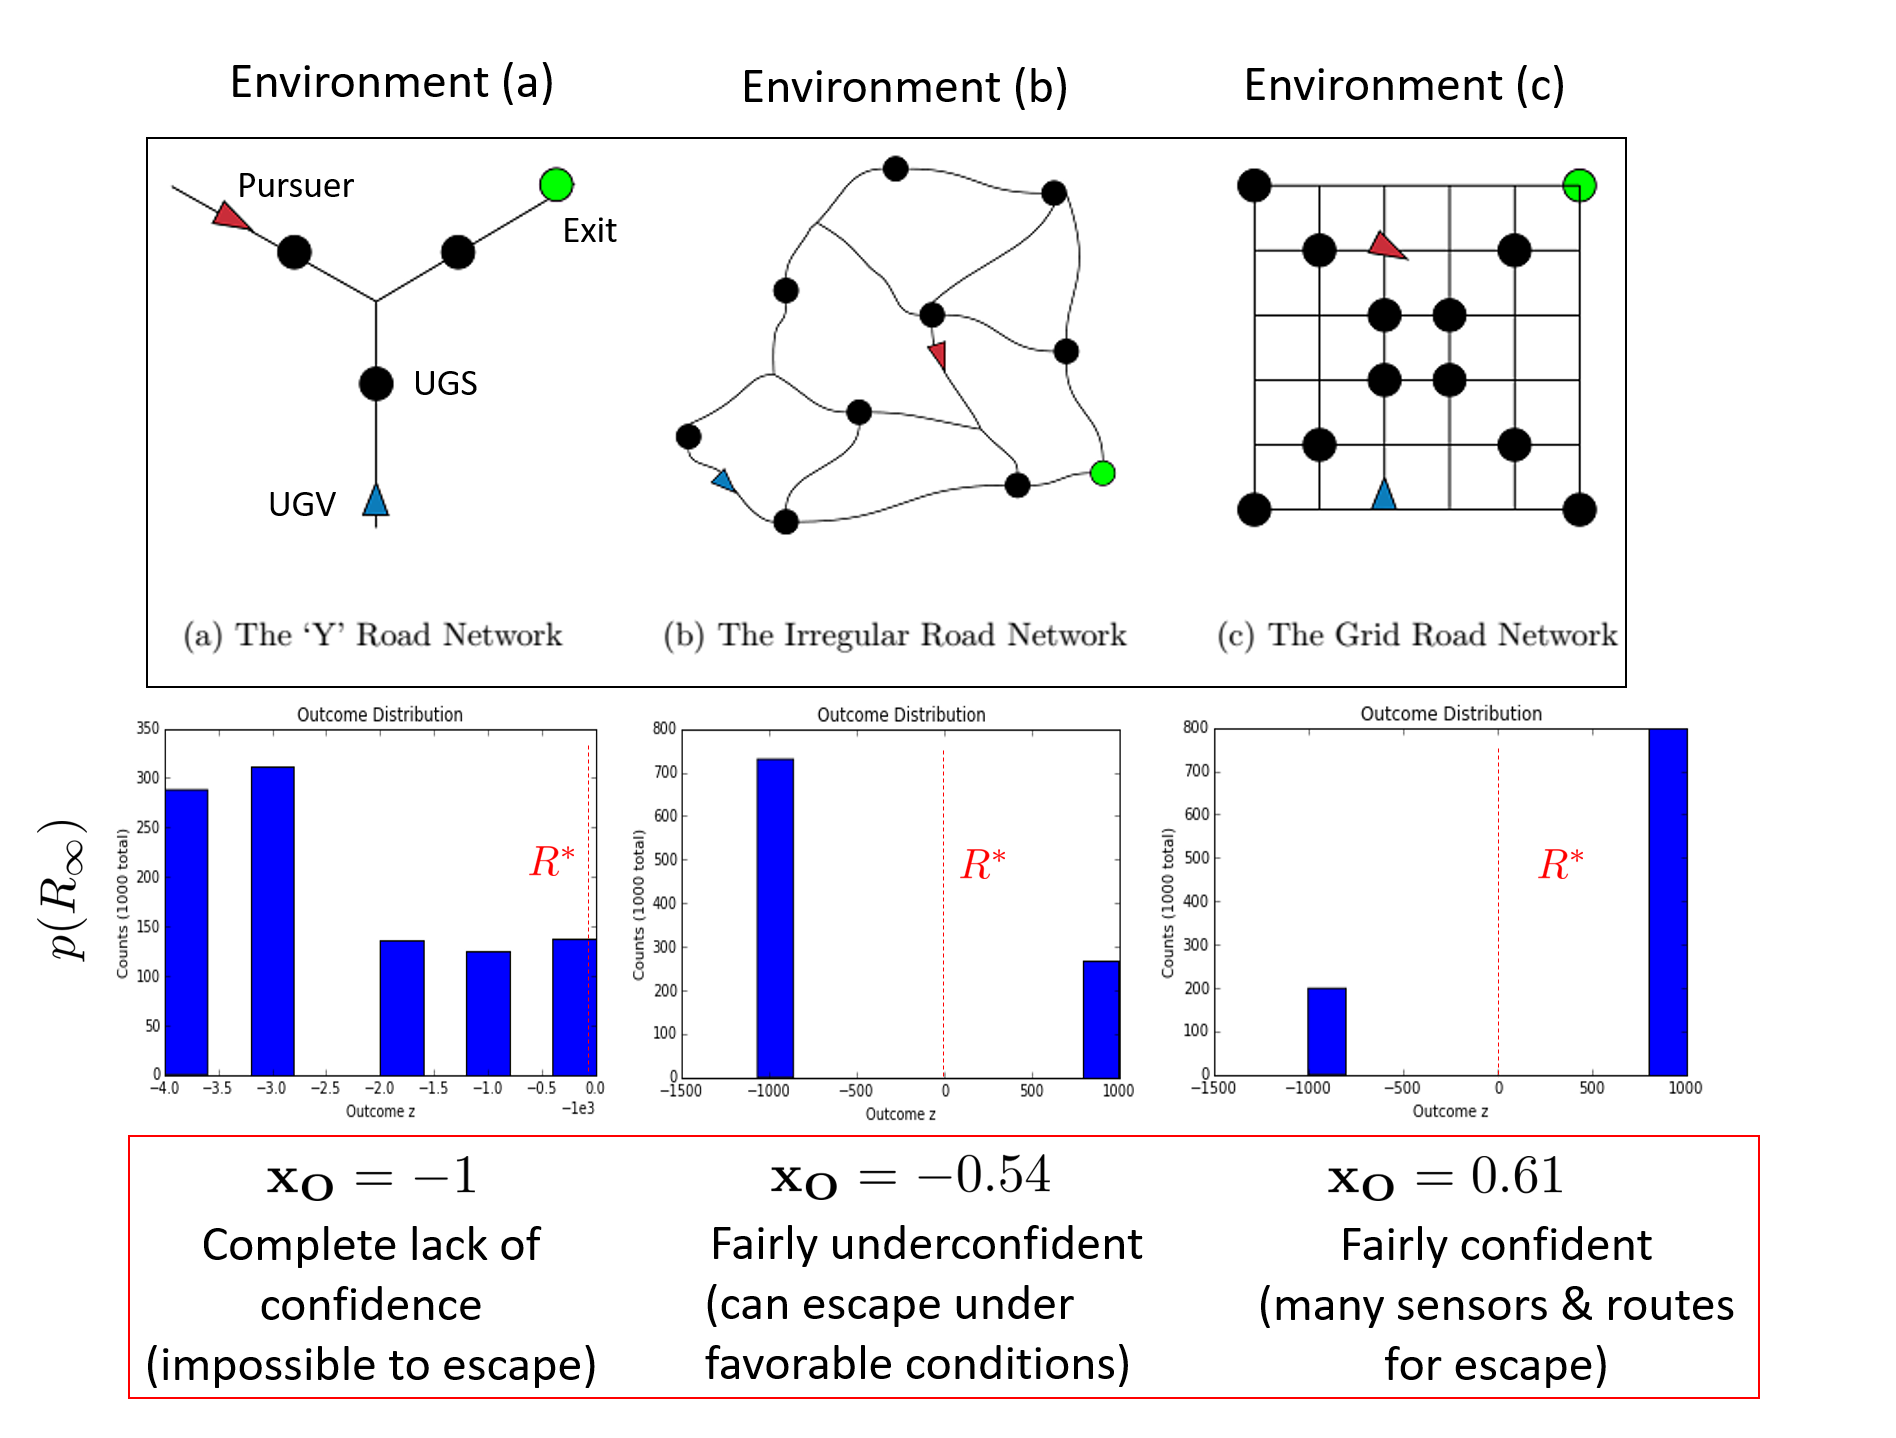
\includegraphics[width=0.68\linewidth]{Figures/xO_envsOnly.png}
        \caption{\xO{} assessments for Donut Delivery problem in various environments.}
        \label{fig:xOexample}
    \end{figure}



However, ref. \cite{Aitken2016-cv} does not specify how to compute other factors, nor how to cope with interdependencies between factors that will arise when assumptions such as those above are relaxed. Furthermore, studies with human users have not yet been done to validate and evaluate the impact of self-confidence reporting on task delegation. The remainder of the paper presents results to address both these gaps. In the next section, we examine how the insights above can be extended to computation and analysis of other \famsec{} factors, focusing here on the solver quality metric \xQ{}. A natural starting point for this is: what can information related to the assessment of \xO{} tell us about how other factors should be assessed? Note that \xO{} indirectly depends on \xQ{}, since reliable estimation of $p_{\pi}(R_{\infty})$ requires knowing the optimal $\pi$. But in practice, an MDP-based APS will often employ an approximate policy $\tilde{\pi}$ instead of the true optimal policy $\pi$. In turn, this leads to an estimate $p_{\tilde{\pi}}(R_{\infty})$ of the expected reward distribution which differs from the true $p_{\pi}(R_{\infty})$ under the optimal $\pi$. We show next that, if a surrogate model for $p_{\pi}(R_{\infty})$ can be found when $\pi$ is unknown but $\tilde{\pi}$ is available, then a quantitative comparison of the estimated $p_{\tilde{\pi}}(R_{\infty})$ to the surrogate $p_{\pi}(R_{\infty})$ leads to a suitable metric for \xQ{} (under the progressively relaxed assumption of \xM{}=+1, \xP{}=+1, and \xI{}=+1). 

\section{Solver Quality Definition and Calculation} \label{sec:SQ}
\nisar{note to self: stopped here...also need to improve technical description: use more conventional phrasing like `surrogate function/model' to describe what is going on with the trusted solver...some of this is used later, but should be used here}
    The factor \xQ{} indicates how well a solver \solve{} will perform on a given (possibly un-encountered) task \task{} of a given class \taskclass{}. 
    \nisar{this should be stated more precisely: how closely the policy produced by a solver \solve{} approximates an optimal/baseline policy or how well it performs relative to an optimal/baseline policy...there is a nuance here in the choice of comparing policies vs. value functions/total expected reward, which is alluded to below but not clearly stated as such...}
    %(i.e. all road networks with a , , and exit, et cetera as described previously). 
    %The need for \xQ{} is not necessarily easy to understand; an analogy helps to clarify: \brett{I have now started thinking about \xP{} being the \emph{shape} of the distribution, and \xQ{} referring to the location of the distribution with respect to the trusted \solvestar{}}
%
    %\emph{Clarifying Example:} One could informally think of \xQ{} as an indication of the \emph{ability} of an athlete. This is opposed to the athlete's assessment of the desirability of the outcome of a game (\xO). While an athlete may be very capable (high \xQ), the score of the game may be such that the athlete knows that it is nearly impossible to catch up and win the game (low \xO). Conversely, an athlete may not be very capable (low \xQ), and due to being na\"{i}ve has an incorrect assessment of the desirability of the outcome (\xO{} cannot be trusted). \nisar{might be best to put this at end/conclusions somewhere to highlight future directions and connections...}
    
    The formal desiderata for \xQ{} are: (\textbf{D1}) reflect competence of solver \solve{} for task \task{}; (\textbf{D2}) enable comparison across solver classes; 
    (\textbf{D3}) extend to unseen tasks of the same class. 
    %\begin{enumerate}[label=\textbf{D\arabic*}]
    %    \item reflect competence of solver \solve{} for task \task{} (where competence is analogous to the `ability' of the athlete in the example)\label{itm:d1}
    %    \item enable comparison across solver classes \label{itm:d2}
    %    \item extend to unseen tasks of the same class \taskclass \label{itm:d3}
    %\end{enumerate}
    
    For practical application, it is critical to be able to compare the quality of solvers of different classes (i.e. exact vs. approximate) because there are many different ways of solving tasks. Likewise, it is also common for an APS to encounter a similar, but previously unseen, task (i.e. a different road network).
    
    \nisar{this should come earlier and be more technically precise/clear...no sense in talking about competence and quality for a few parags if these are not defined up front!} 
    Evaluating the `quality' of something implies some kind of comparison is taking place. In this setting the desired comparison is between a `candidate solver' \solve{} and some reference solver. Ideally, the candidate solver could be compared to the exact solution (whose quality is by definition perfect), but there are three main challenges: 1) It is unclear how policies/solvers should be compared; 2) Large state spaces make exact solutions infeasible; and 3) It is generally impossible to evaluate the exact solution for \emph{all} tasks of a given task class \taskclass{} (linked to \ref{itm:d3})
        %
    % \subsubsection{Summary} The comparison of policies will be done through comparing reward distributions; this approach addresses both \ref{itm:d1} and \ref{itm:d2}, along with \ref{itm:l1}. In order to address \ref{itm:l2}, \ref{itm:l3}, and \ref{itm:d3} a `trusted solver' \solvestar{} will be introduced to serve as a basis by which a `candidate solver' \solve{} can be evaluated. Furthermore, a surrogate model \surrogate{} will be learned to predict \rwdstarapprox{} on un-encountered tasks. In this way, all desiderata, and challenges have been addressed.
    \begin{figure}[tb]
        \centering
        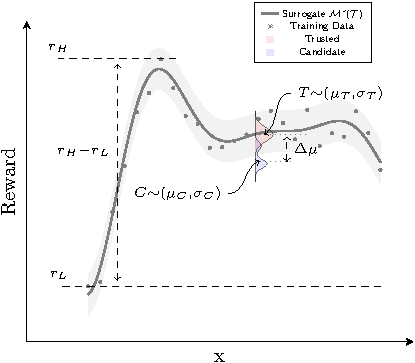
\includegraphics[width=0.6\linewidth]{Figures/sq_v2_fig-crop}
        \caption{Key values involved in calculating \xQ, where $x$ represents a `parameter of interest' for task \task, or solver \solve.}
        \label{fig:sq_v2}
        \vspace{-0.2cm}
    \end{figure}
